\documentclass[a4paper]{jarticle}
\usepackage{sice-si}
\usepackage{amsmath} 
\usepackage[dvipdfmx]{graphicx}


\begin{document}
%
% タイトルと著者名
\title{音声中に出現する特定キーワードの自動ゲイン調整を行う装置の開発} % 和文タイトル
\name{○佐々部 岳人,天野 俊一(流通経済大学)} % 著者名
\etitle{Development of a device that automatically adjusts the gain of specific keywords that appear in speech.} % 英文タイトル
\ename{○Gakuto Sasabe, and Shunichi Amano (Ryutsu Keizai University)}	%著者名(英)
%
% アブストラクト
\abst{
When we obtain information visually, it is possible to filter only the information we want to obtain, for example, by using a recommendation function for online shopping. On the other hand, in the auditory sense, technologies that uniformly cut noise in specific frequency bands in the outside world, such as noise cancellation, have been put to practical use, but there are still few technologies that cut specific information such as keywords that appear in speech. If such technology is put to practical use, it is expected to contribute to the improvement of productivity and creativity in work involving listening. In this study, we will develop a system that automatically adjusts the gain of speech corresponding to specific keywords. We will also examine the effect of this system on the user's task performance.
}
% タイトルの出力
\maketitle
%
% 本文
\section{緒言}
本稿では SICE SI 部門講演会 SI の予稿原稿を作成するための説明を行います.
SIでは予稿原稿としてPDFファイル形式のファイルを電子投稿していただくことを原則とさせていただいております.
ただし,電子化やネットワーク接続が困難な場合には個別に対応させていただきますので,プログラム委員会までご相談ください(Webサイトからお問い合わせできます).
%
\section{自動ゲイン調整装置}
\subsection{装置の構成}
\begin{figure}[htbp]
    \begin{center}
    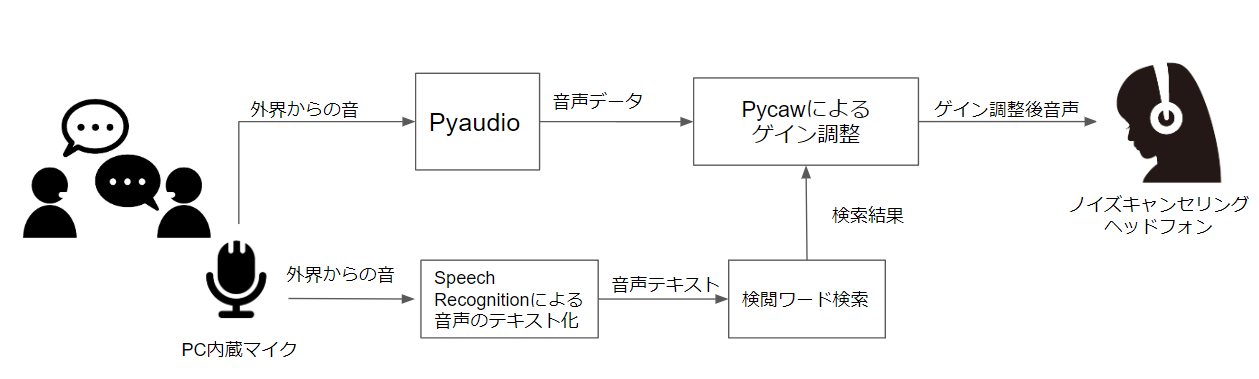
\includegraphics[width=80mm]{system.PNG}
    \caption{The device and the configuration.}
    \label{fig:system}
    \end{center}
    \end{figure}
本稿で使用した装置の構成をFig.\ref{fig:system}に示す.
本装置はワイヤレスノイズキャンセリングヘッドフォン,PC,マイクによって構成される.
PCの中に,Pythonで書かれたシステムが搭載されており,これによってマイクからの音に対して自動でゲイン調整を行う.
以下に,マイクから音を拾って,ユーザーがゲイン調整された音を聞くまでのシステム内の流れを示す.
まず,外界からの音をマイクによって拾い,Google社のSpeech recogntionによってノイズ処理と音声のテキスト化が行われる.
次に,生成されたテキストは検閲ワード検索クラスに送られ,あらかじめ設定された検閲ワードがテキスト中に含まれていないかどうか検索が行われる.
もし,テキスト中に検閲ワードが含まれていた場合は,「検閲ワードあり」の情報がゲイン調整クラスに送られる.
一方で,外界からの音はPythonライブラリであるPyaudioによってチャンクごとの音声データに分けられる.(Fig.\ref{fig:system}の上部分)

    
\section{ゲイン調整システムの検証実験}
\subsection{システムによる音のカットの確認}
\subsubsection{実験概要}
\subsubsection{実験結果}
\subsection{システムがタスク遂行に与える影響}
\subsubsection{実験概要}
\subsubsection{実験結果}
\section{ディスカッション}
%
%
%参考文献
\begin{thebibliography}{99}
\bibitem{SI}
	計測太郎,制御花子:
	``SICE SI予稿原稿の書き方(サンプル)'',  
   {\it 計測自動制御学会SI部門講演会SICE-SI予稿集}, 
    pp.0000--0000 (20??)
\end{thebibliography}
%
%
%
\end{document}

